% Options for packages loaded elsewhere
\PassOptionsToPackage{unicode}{hyperref}
\PassOptionsToPackage{hyphens}{url}
%
\documentclass[
]{book}
\usepackage{amsmath,amssymb}
\usepackage{iftex}
\ifPDFTeX
  \usepackage[T1]{fontenc}
  \usepackage[utf8]{inputenc}
  \usepackage{textcomp} % provide euro and other symbols
\else % if luatex or xetex
  \usepackage{unicode-math} % this also loads fontspec
  \defaultfontfeatures{Scale=MatchLowercase}
  \defaultfontfeatures[\rmfamily]{Ligatures=TeX,Scale=1}
\fi
\usepackage{lmodern}
\ifPDFTeX\else
  % xetex/luatex font selection
\fi
% Use upquote if available, for straight quotes in verbatim environments
\IfFileExists{upquote.sty}{\usepackage{upquote}}{}
\IfFileExists{microtype.sty}{% use microtype if available
  \usepackage[]{microtype}
  \UseMicrotypeSet[protrusion]{basicmath} % disable protrusion for tt fonts
}{}
\makeatletter
\@ifundefined{KOMAClassName}{% if non-KOMA class
  \IfFileExists{parskip.sty}{%
    \usepackage{parskip}
  }{% else
    \setlength{\parindent}{0pt}
    \setlength{\parskip}{6pt plus 2pt minus 1pt}}
}{% if KOMA class
  \KOMAoptions{parskip=half}}
\makeatother
\usepackage{xcolor}
\usepackage{longtable,booktabs,array}
\usepackage{calc} % for calculating minipage widths
% Correct order of tables after \paragraph or \subparagraph
\usepackage{etoolbox}
\makeatletter
\patchcmd\longtable{\par}{\if@noskipsec\mbox{}\fi\par}{}{}
\makeatother
% Allow footnotes in longtable head/foot
\IfFileExists{footnotehyper.sty}{\usepackage{footnotehyper}}{\usepackage{footnote}}
\makesavenoteenv{longtable}
\usepackage{graphicx}
\makeatletter
\def\maxwidth{\ifdim\Gin@nat@width>\linewidth\linewidth\else\Gin@nat@width\fi}
\def\maxheight{\ifdim\Gin@nat@height>\textheight\textheight\else\Gin@nat@height\fi}
\makeatother
% Scale images if necessary, so that they will not overflow the page
% margins by default, and it is still possible to overwrite the defaults
% using explicit options in \includegraphics[width, height, ...]{}
\setkeys{Gin}{width=\maxwidth,height=\maxheight,keepaspectratio}
% Set default figure placement to htbp
\makeatletter
\def\fps@figure{htbp}
\makeatother
\setlength{\emergencystretch}{3em} % prevent overfull lines
\providecommand{\tightlist}{%
  \setlength{\itemsep}{0pt}\setlength{\parskip}{0pt}}
\setcounter{secnumdepth}{5}
\usepackage{booktabs}
\usepackage{fancyhdr}
\pagestyle{fancy}


\usepackage{xstring}
\usepackage{catchfile}
\CatchFileDef{\HEAD}{.git/refs/heads/master}{}
\newcommand{\gitrevision}{%
  \StrLeft{\HEAD}{7}%
}


% center of header
\fancyhead[CO,CE]{}
% center of footer
\fancyfoot[CO,CE]{\gitrevision}
% page number on the left of even pages and right of odd pages
\fancyfoot[LE,RO]{\thepage}


\ifLuaTeX
  \usepackage{selnolig}  % disable illegal ligatures
\fi
\usepackage[]{natbib}
\bibliographystyle{plainnat}
\usepackage{bookmark}
\IfFileExists{xurl.sty}{\usepackage{xurl}}{} % add URL line breaks if available
\urlstyle{same}
\hypersetup{
  pdftitle={FlowMax-Q Manual},
  pdfauthor={Srirama Bhamidipati},
  hidelinks,
  pdfcreator={LaTeX via pandoc}}

\title{FlowMax-Q Manual}
\author{Srirama Bhamidipati}
\date{Last Updated 2024-03-08 15:17:25 Asia/Calcutta}

\begin{document}
\maketitle

{
\setcounter{tocdepth}{1}
\tableofcontents
}
\chapter*{Preface}\label{preface}
\addcontentsline{toc}{chapter}{Preface}

This manual\footnote{Version \textbf{d99dce5}} is divided into two parts. Part I deals with handling FlowMax network (nodes and edges) in a QGIS environemnt and Part II deals with using the FlowMax-Q, a QGIS plugin to work with outputs from FlowMax.

\part{Editing in QGIS}\label{part-editing-in-qgis}

\chapter{Introduction}\label{introduction}

\begin{itemize}
\tightlist
\item
  Economy based scenarios are to be modified in the trade-databases.
\item
  Resilience based scenarios (GIS) fall into 2 categories:

  \begin{itemize}
  \tightlist
  \item
    node-based

    \begin{itemize}
    \tightlist
    \item
      editing geometries;
    \item
      editing attributes
    \end{itemize}
  \item
    edge-based

    \begin{itemize}
    \tightlist
    \item
      editing geometries;
    \item
      editing attributes
    \end{itemize}
  \end{itemize}
\item
  Technology based scenarios will affect the demand (freight composition)
\item
  Policy based scenarios will affect the route and mode choices (freight composition)
\end{itemize}

\chapter{Scenarios}\label{scenarios}

The image below shows the underlying structure of constructing scenarios

\begin{figure}
\centering
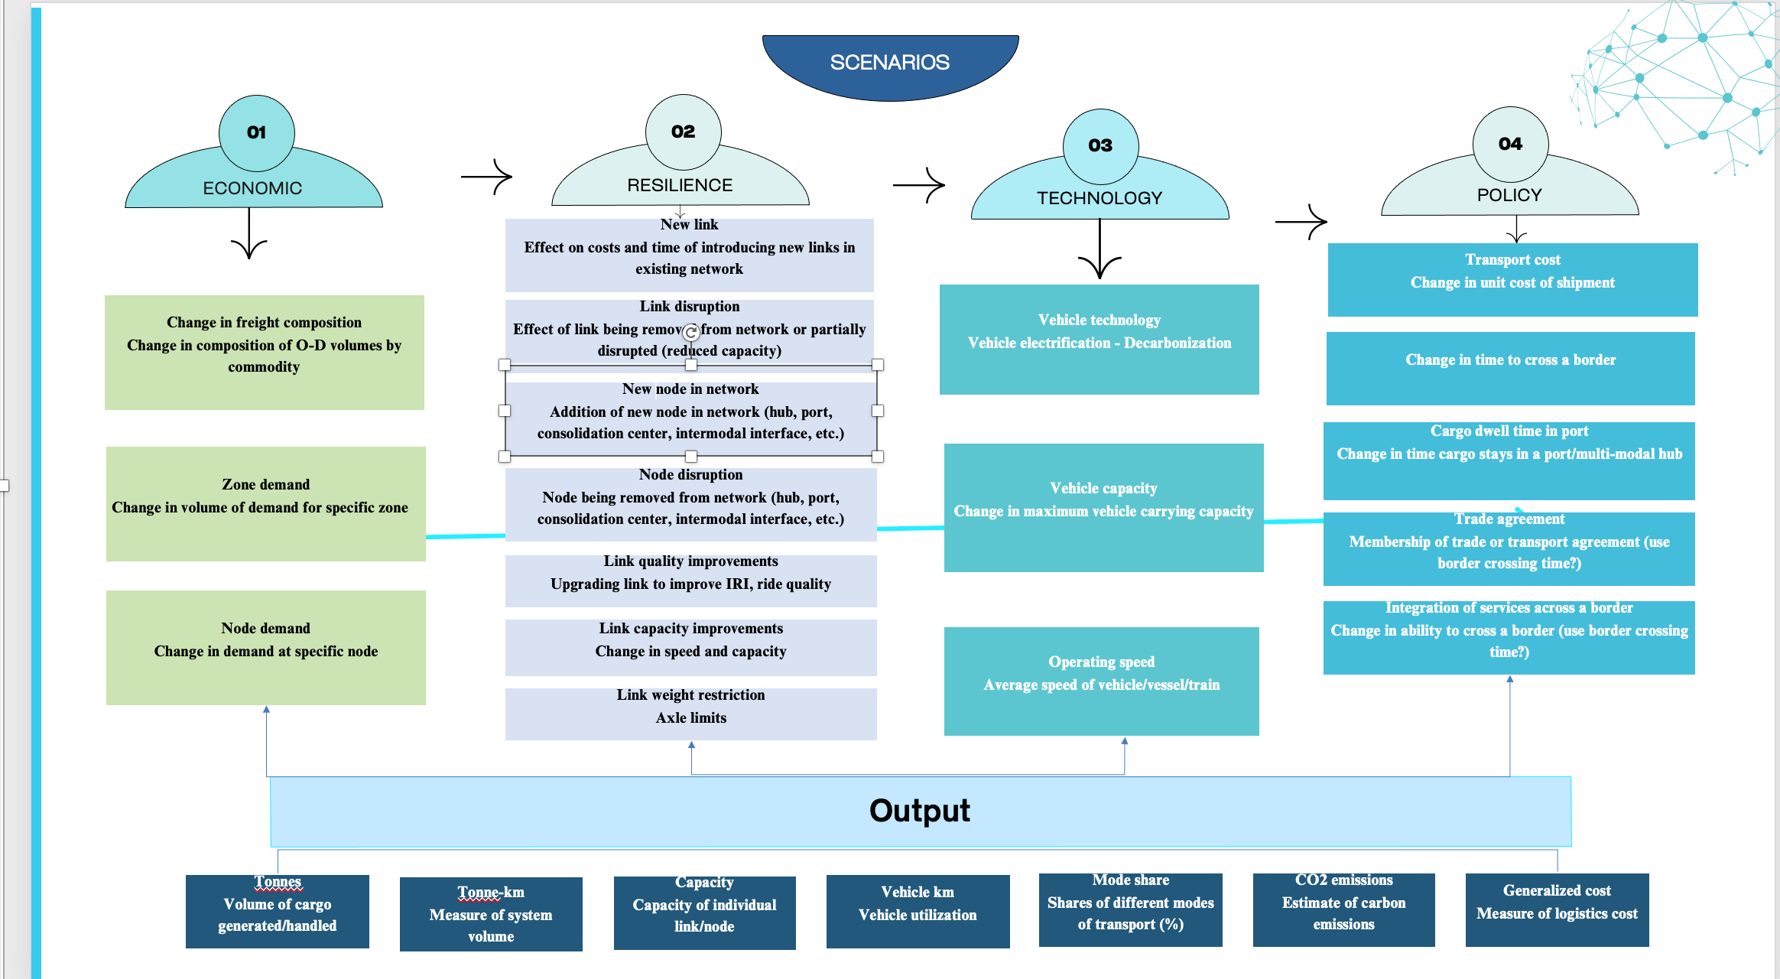
\includegraphics{images/Picture1.png}
\caption{Scenarios}
\end{figure}

\chapter{Adding Links}\label{adding-links}

\section{Connect to an non-existing node}\label{connect-to-an-non-existing-node}

Is there an existing node at the source or destination of this (to be added) new link?

\begin{itemize}
\tightlist
\item
  No? First create a node(s) and then create a line between source and destination nodes.
\item
  Yes ? Create a line between source and destination nodes.
\end{itemize}

\section{Connect to an existing node}\label{connect-to-an-existing-node}

Is the new link connecting to an existing node location?

\begin{itemize}
\tightlist
\item
  Create a line between source and destination nodes.
\end{itemize}

\section{Adding links - Hands-on}\label{adding-links---hands-on}

\begin{itemize}
\tightlist
\item
  Check the highest node number (NodeID\textsubscript{H}) from the node file. To do this, open the attribute table of the shapefile \textbf{Right Click on the node layer\textgreater{} Open Attribute Table} . Scroll if required to see the NodeID field, \textbf{Click on the field heading} to sort the column in ascending or descending order. When in descending order, make note of the top most row to identify the current highest node number.
\item
  Set the node file in edit mode, and add a node (point geometry) to the node file and assign it a node number = NodeID\textsubscript{H}+1
\item
  Fill in all other node attribute columns as necessary (\hyperref[modifying-node-attributes]{see also})
\item
  Save edits and stop the edit mode on node file.
\item
  Check the highest edge number (EdgeID\textsubscript{H}) from the link file.
\item
  Set the link file in edit mode and add a link (line-geometry) from existing node to the new node created in step 2, assign this link an edge number = EdgeID\textsubscript{H} + 1
\item
  Fill in all other link attribute columns as necessary (\hyperref[modifying-edge-attributes]{see also})
\item
  Save edits and stop the edit mode on link file
\end{itemize}

\chapter{Removing Links}\label{removing-links}

Removing links is easier than adding links. It is recommended to disable links than to delete them.

\chapter{Modifying Node Attributes}\label{modifying-node-attributes}

\chapter{Modifying Edge Attributes}\label{modifying-edge-attributes}

\part{QGIS Plugin}\label{part-qgis-plugin}

\chapter{Installing the plugin}\label{installing-the-plugin}

\end{document}
